\documentclass[../main.tex]{subfiles}
\begin{document}

\section{Können Computer denken?}
Ob Computer denken können ist aus Sicht der Abhängigkeit der Welt von ihnen immer wichtiger. Zusätzlich, insbesondere vom Standpunkt der Philosophie, ist die Frage nach dem Denkprozess und was ihn ausmacht von grosser Bedeutung. 

\paragraph{Defintion von Denken} ist wie folgt: Man kann denken, wenn man (1) in der Lage ist, Gedanken, Überzeugungen/Meinungen und andere mentale Zustände auszubilden und (2) Überlegungen anstellen/Schlüsse ziehen kann. 

\section{Computer und Computationale Theorien des Geistes}
\subsection{Die Turingmaschine}
Die Turingmaschine ist der Urvater der Computer und nach wie vor repräsentativ für die theoretische Funktionsweise aller Computer. Er wurde von Alan Turing (1912-1954) erfunden. 

Die Turingmaschine besteht aus drei Elementen: Einer Kontrolleinheit, die eine endliche Zahl von internen Zuständen annehmen kann, einem beidseitig unendlichen, eindimensionalen Speicherband, welches in Zeichenfelder unterteilt ist und einem Schreib-Lese-Kopf. 

\begin{figure}[!htb]
\centering
{\centering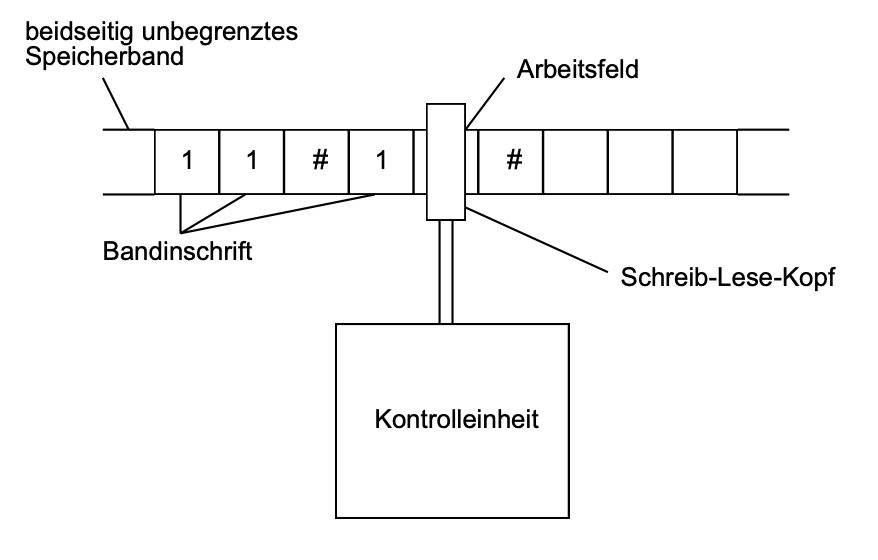
\includegraphics[height=6cm]{images/turing_maschine.png}\endcenter}
\caption{Gemäss Folie aus der Vorlesung}
\end{figure}


Die Turingmaschine ist deshalb relevant, weil sie \textbf{jedes Problem} lösen kann, das auch durch einen Computer gelöst werden kann. Oder in anderen Worten: Die Turingmaschine \textit{ist} ein Computer. 

\subsubsection{Einfache Aufgabe}
Angenommen man will mit der Turingmaschine zwei unäre Terme (<<1>> --> <<1>>, <<2>> --> <<11>>, <<3>> --> <<111>>) addieren, geschieht das wie folgt. Der Term ist <<111+11>> (= 3 + 2). Gestartet wird auf dem ersten <<1>> des Terms. Das Resultat ist <<11111>> ( = 5).

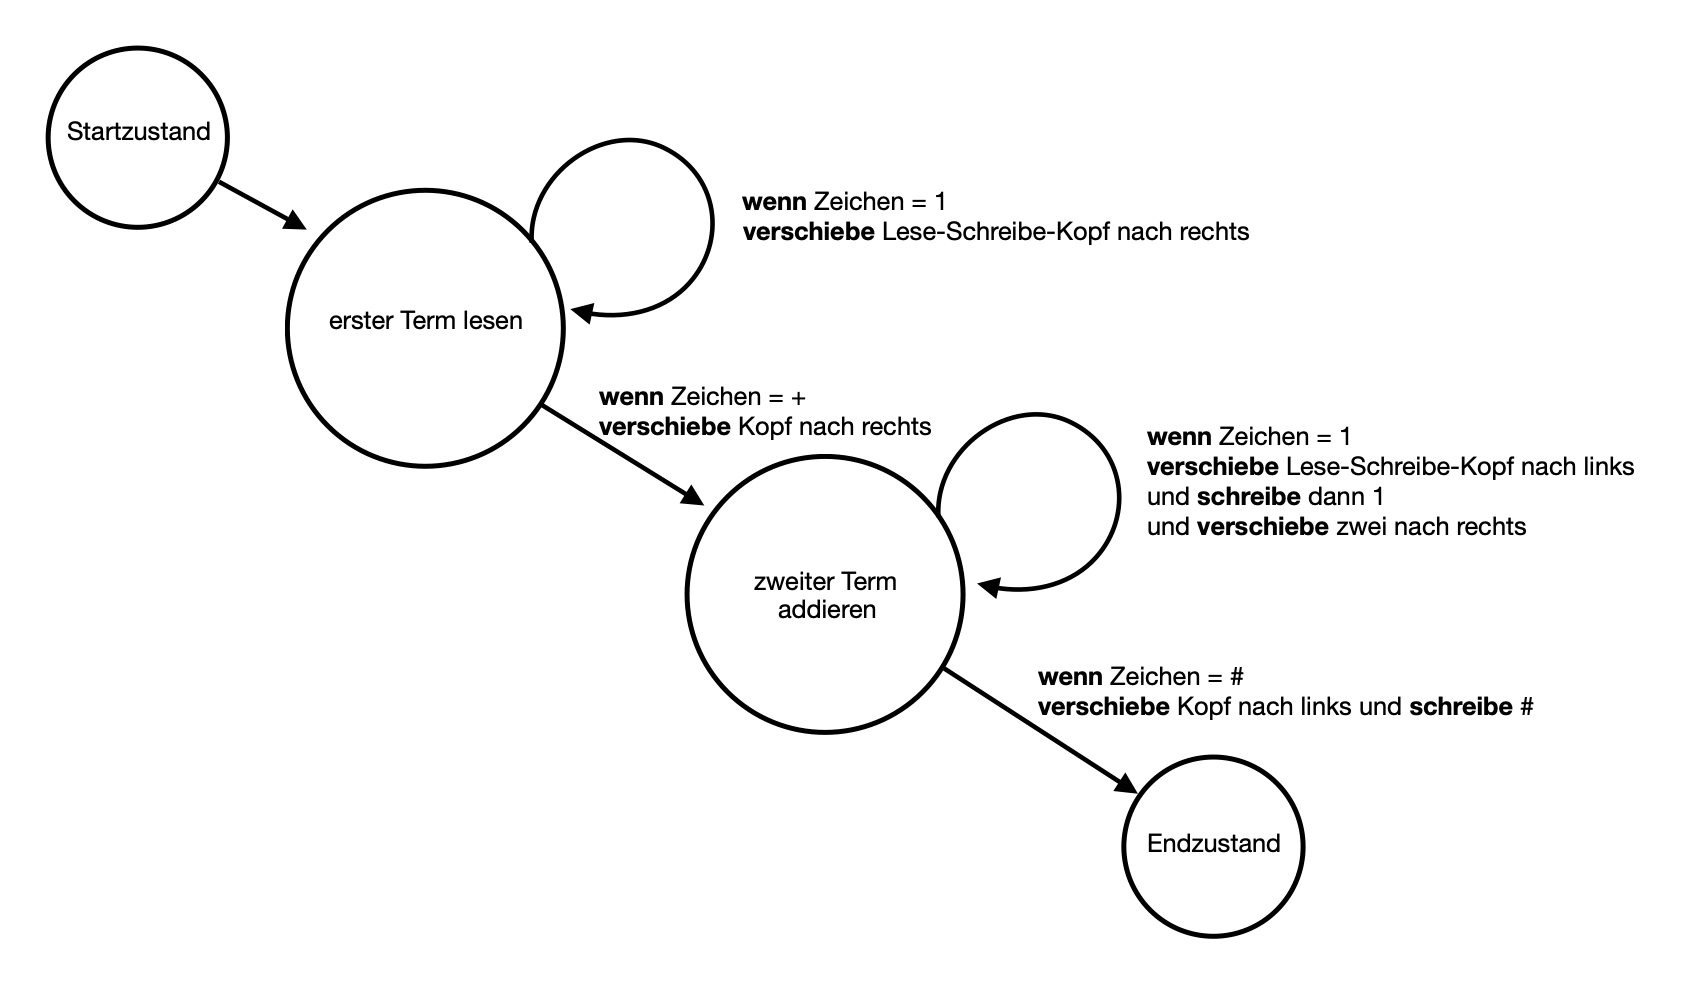
\includegraphics[width=\textwidth]{images/turingmaschine_unaere_terme_addieren.png}

\subsection{Computationale Theorien des Geistes}
Die Grundidee von computationalen Theorien des Geistes besagt, dass Denkprozesse gleich sind wie computationale Prozesse (schrittweise Symbolverarbeitung und Manipulation von Zeichenketten). Unser Denkprozess unterscheidet sich aber von Computern insofern, dass der Computer mit elektrischen Signalen und das Gehirn (vermutlich) mit neuronalen Aktivationsmustern funktioniert. 

Computationale Theorien, deren Vertreter aus verschiedenen Bereichen kommen (Jerry Fodor aus der Philosophie, Zenon Pylyshyn aus der Psychologie, Allen Newell aus der Informatik, Herbert Simon aus der Politikwissenschaften), werden unterschieden in \textbf{schwache Versionen}, die besagen, dass der Denkprozess computationale Prozesse involviert (notwendig, aber nicht hinreichend für Denkprozesse), und \textbf{starke Versionen}, die besagen, dass der Denkprozess \textit{allein} durch das Vorhandensein eines (komplexen) computationalen Prozesses gegeben ist (sind notwendig und hinreichend für Denkprozess). Die starke Version wird jedoch kaum vertreten!

\paragraph{Einschränkungen} Als computationale Denkprozesse zählen nur die Denkprozesse, die mit der Umwelt agieren (also aufgrund von Inputs stattfinden oder Outputs erzeugen). Zusätzlich muss ein computationales System eingebettet sein, um ein denkendes System zu sein. 

\section{Das Argument vom chinesischen Zimmer}  
Das Argument versucht aufzuzeigen, dass weder heutige noch zukünftige Computer in der Lage sind, denken zu können. Damit widerlegt es die <<starke KI-These>>. 
\subsection{Experiment}
Angenommen wir befänden uns in einem Zimmer voller Regelbücher über die Chinesische Sprache, die wir selber nicht beherrschen. Durch eine Durchreiche erhalten wir Schrifttafeln mit Chinesischen Zeichen, die wir, aufgrund der Regelbücher, erweitern und wieder herausgeben. 

Es lässt sich beobachten, dass wir, obschon wir korrekte Zeichensätze herausgeben können, nicht verstehen, \textit{was} die Bedeutung dieser ist. Wir können also schlussfolgern, dass wir nicht aufgrund der korrekten Funktionsweise schlussfolgern können, dass Verständnis vorhanden ist. 

Anders ausgedrückt: \textbf{Die Manipulation von Symbolen nach syntaktischen Regeln ist nicht hinreichend dafür, den Symbolen eine Bedeutung zu verleihen. Verstehen und Denken erfordert also Zustände mit Bedeutung} (semantischem Gehalt).

\paragraph{Einwände zum Experiment}
\begin{enumerate}
	\item Das System besteht nicht nur aus der Person im Zimmer, sondern aus dem ganzen Zimmer inkl. dessen Inhalt (Bücher + Person). Dieses versteht sehrwohl Chinesisch. 
		
		Searles Antwort: Wenn die Person kein Chinesisch versteht, dass ist offensichtlich, dass auch das System Person+Zimmer kein Chinesisch versteht. 
	\item Zwar versteht ein System nicht alleine aufgrund der Tatsache, dass man Konversationen abbilden kann, Chinesisch, aber wenn dieses System in einen Roboter eingebaut ist, dessen interne Mechanismen äussere Sachverhalte mit ihren Kausalbeziehungen verstehen, versteht dieser Chinesisch, wenn er das Programm ausführt. 
		
		Searles Antwort: Angenommen man stellt sich das Zimmer und die Person verkleinert in einem Kopf vor und angenommen die Outputs aus dem Zimmer lösen Handlungen aus, dann kann nach wie vor noch nicht von Verstehen von Bedeutungen geredet werden (Output hat keinen semantischen Gehalt), und deswegen kann nicht von Denkprozessen gesprochen werden. 
\end{enumerate}

\end{document}